SelfBACK HAR data set has been recorded by 34 users performing 6 activities while wearing accelerometer on wrist and accelerometer on thigh. Table \ref{table:dataset} is a summary of the dataset characteristics. The goal of this series of experiments is to find if accelerometer data from wrist and thigh can improve classification compared to wrist or thigh.

\begin{table}[ht]
\caption{SelfBACK HAR Dataset}
\label{table:dataset}
\begin{center}
\begin{tabular}{|c|c|} 
  \hline
  Number of users & 34 \\
  \hline
  Activities & Standing, Sitting, Walking, Upstairs, Downstairs, Jogging \\
  \hline
  Sensors & Accelerometers on wrist and thigh \\
  \hline
  Sampling rate & 100Hz \\
  \hline
\end{tabular}
\end{center}
\end{table}

\section*{Previous Work}
\label{sec:old}
Results from previous work on this dataset by \citeasnoun{sani2017learning} is summarised in Table \ref{table:results1}. Main conclusion we draw is that thigh accelerometer is a better source of data for HAR compared to wrist. High degree of freedom of wrist unrelated to the activity being performed contributes as noise and interfere with classification. 

\begin{table}[ht]
\caption{SelfBACK classification task with single sensor}
\label{table:results1}
\begin{center}
\begin{tabular}{|c|c|c|} 
  \hline
  \multirow{2}{*}{Classification task} & \multicolumn{2}{|c|}{F1 measure} \\\cline{2-3}
  & Wrist & Thigh \\
  \hline
  CNN-SVM & 0.850 & 0.957 \\
  \hline
  CNN-kNN & 0.845 & 0.949 \\
  \hline
  CNN & 0.839 & 0.959 \\
  \hline
  DCT-SVM & 0.836 & 0.967 \\
  \hline
\end{tabular}
\end{center}
\end{table}

\section*{Sensor Fusion}
\label{sec:fusion}
We conducted number of experiments to evaluate the effect of fusion between two accelerometer data from wrist and thigh. We used window size of 300 time stamps (3 second window) as input and performed Leave-one-user-out (LOUO) through out this series of experiments and present average accuracy from 34 experiments. We compare all experiments against the baselines of single sensor architectures. All our results are based on three layer convolution architecture for each individual CNN although figures show one convolution for clarity. Three layers are of 150, 100 and 60 feature maps maintaining consistency with the pyramid architecture introduced by \citeasnoun{sani2017learning}. These hyper-parameters were finalized after testing with different number of layer and number of feature maps.

First we explore fusion architectures to observe how fusion of these two sensor streams affect classification accuracy. Fist we learn feature embeddings of two sensors from individual CNNs, then fuse fuse feature embeddings with concatenation (concat) as two feature maps (Figure \ref{fig:concat}). Each input is shaped as one dimensional input of length 300 and three axis were used as 3 channels. Results are presented in Table \ref{table:fusion1}.

\begin{figure}[ht]
\centering
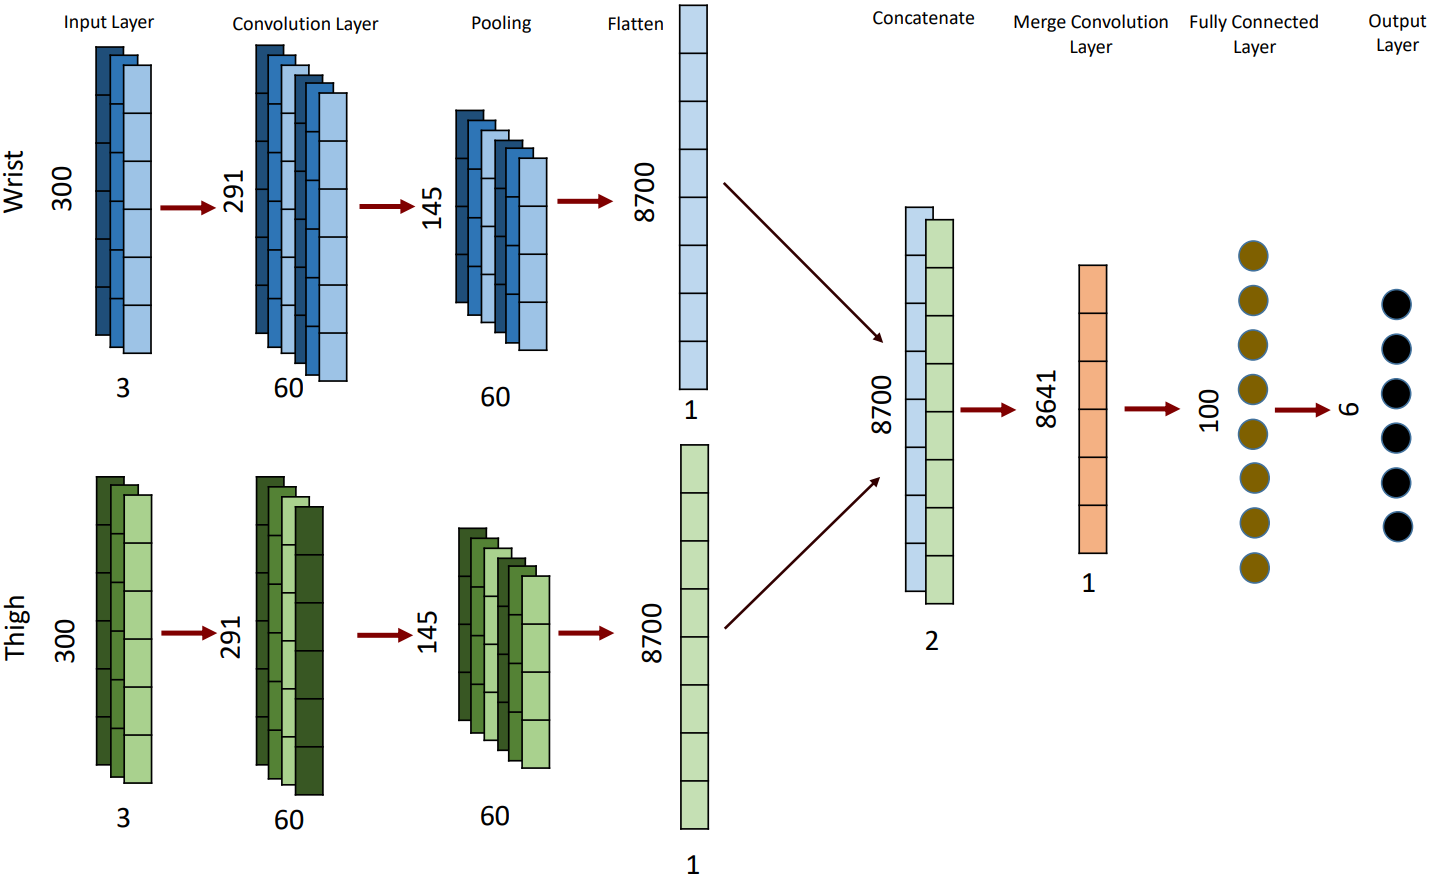
\includegraphics[width=0.5\textwidth]{concat}
\caption{Sensor Fusion Architecture with one convolution layer}
\label{fig:concat}
\end{figure}

\begin{table}[ht]
\caption{Results: Sensor Fusion architectures }
\label{table:fusion1}
\begin{center}
\begin{tabular}{|c|c|} 
  \hline
  Architecture & Test Accuracy \\
  \hline
  Wrist & 86.04738529 \\
  \hline
  Thigh & 96.44364706 \\
  \hline
  Fusion with concatenation layer & 95.94770249 \\
  \hline
\end{tabular}
\end{center}
\end{table}

We also treated each sensor axis as one input and results can be found on Table \ref{table:fusion2}. When treating each axis as one input, in the baseline model for wrist there are three individual convolutions going in to concatenation layer and in the fusion architecture there are 6 independent convolutions for each axis (Figure \ref{fig:channelconcat}).  

\begin{figure}[!ht]
\centering
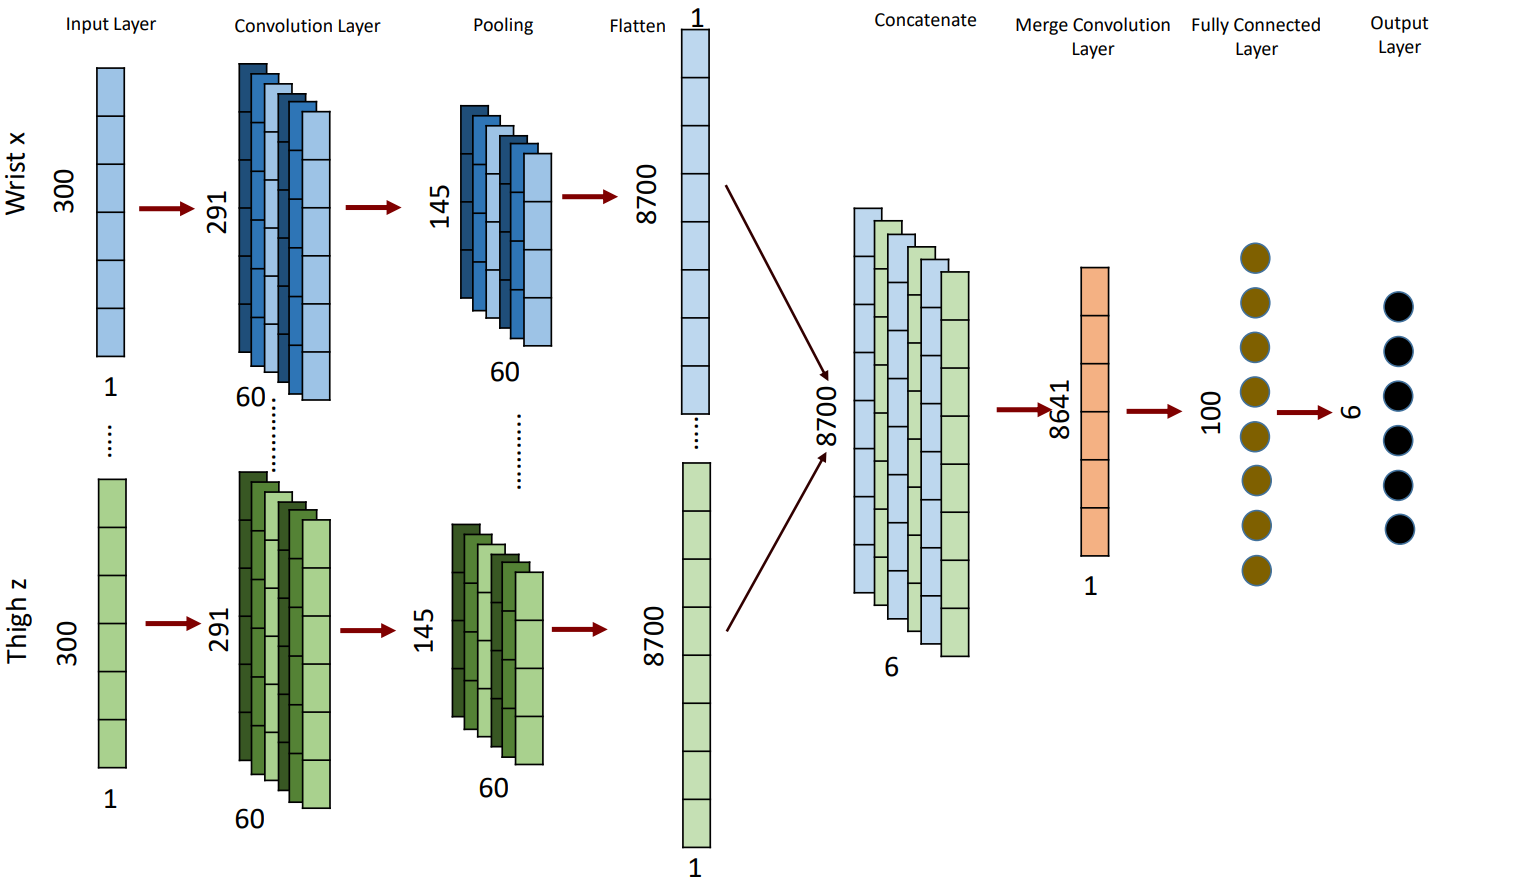
\includegraphics[width=0.5\textwidth]{conca_6}
\caption{Axis Fusion Architecture with one convolution layer}
\label{fig:channelconcat}
\end{figure}

\begin{table}[!ht]
\caption{Results: Axis Fusion architectures }
\label{table:fusion2}
\begin{center}
\begin{tabular}{|c|c|} 
  \hline
  Architecture & Test Accuracy \\
  \hline
  Wrist & 86.33278626 \\
  \hline
  Thigh & 95.99085818 \\
  \hline
  Fusion with concatenation layer & 95.96295427 \\
  \hline
\end{tabular}
\end{center}
\end{table}

From results on Table \ref{table:fusion2} we can conclude treating accelerometer data as different channels or different convolutions does not make a significant difference in performance. More importantly we can see, fusion of wrist and thigh accelerometer data does not improve overall performance of thigh accelerometer data classification.

\section*{Privileged Learning}
Next we explore opportunities of improving wrist performance with thigh data. We have already concluded that wrist is a noisy source of data (section \ref{sec:old}), but wrist is a non intrusive and familiar place to wear a sensor compared to thigh. We want to see if training a model with wrist and thigh data can make a model learn to make better decisions with just wrist data. 

We explore Privileged Learning concept with above purpose. Curriculum Learning was adapted from \citeasnoun{havaei2016hemis} to make the fusion architecture more robust to not having thigh data at test time. The curriculum strategy is we gradually decrease the number of thigh instances the model sees during 100 epochs of training. We try different drop patterns as shown in Figure\ref{fig:CLdrop} and their performance is shown in Figure \ref{fig:CLresult}

\begin{figure}[!ht]
\centering
\begin{subfigure}{.5\textwidth}
  	\centering
  	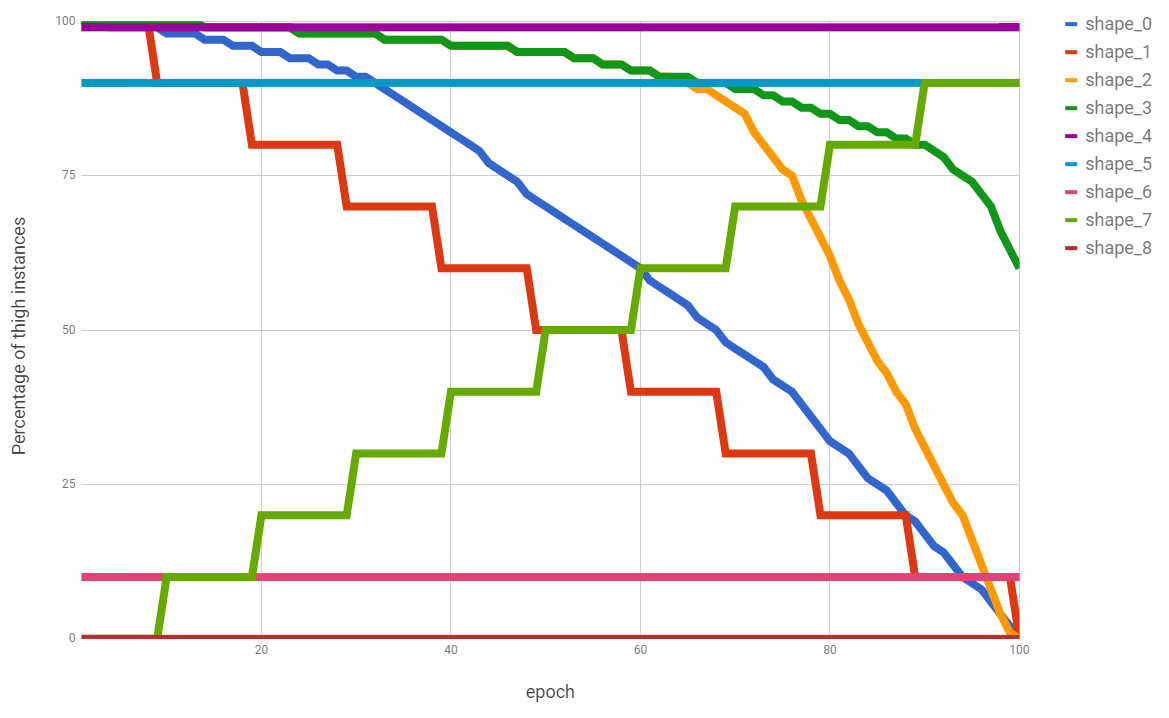
\includegraphics[width=0.8\textwidth]{curr_shapes}
	\caption{Thigh instances drop patterns}
	\label{fig:CLdrop}
\end{subfigure}%
\begin{subfigure}{.5\textwidth}
  	\centering
	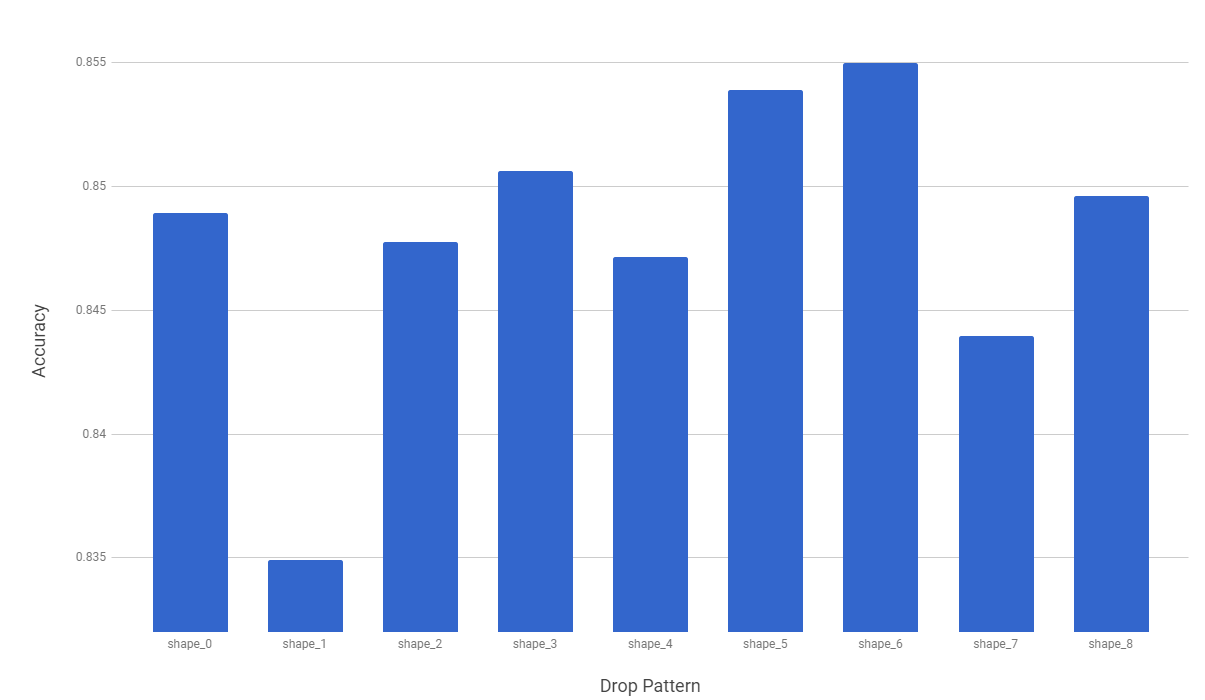
\includegraphics[width=0.8\textwidth]{curr_data}
	\caption{Results}
	\label{fig:CLresult}
\end{subfigure}
\caption{Curriculum Learning Strategies}
\label{fig:test}
\end{figure}

We can observer that dropping thigh 100 percept at all epochs during training provide significantly close performance to having thigh data. Therefore we conclude that wrist and thigh accelerometer data does not improve each-other. 

\clearpage
